\documentclass[conference]{IEEEtran}

\usepackage{amsmath}
\usepackage{graphicx}
%\usepackage[backend=bibtex,style=chem-rsc]{biblatex}
\usepackage{lettrine}
\usepackage{cite}
\usepackage{float}
\usepackage{blindtext}
\usepackage{eso-pic}
\usepackage[utf8]{inputenc}
\usepackage[english]{babel}
\usepackage[numbers]{natbib}
\usepackage{hyperref}
\usepackage{booktabs}
\usepackage{filecontents}
\newcommand\tab[1][1cm]{\hspace*{#1}}
\newcommand\AtPageUpperMyright[1]{\AtPageUpperLeft{%
    \put(\LenToUnit{0.5\paperwidth},\LenToUnit{-1cm}){%
     \parbox{0.5\textwidth}{\raggedleft\fontsize{9}{11}\selectfont #1}}%
    }}%
    \newcommand{\conf}[1]{%
    \AddToShipoutPictureBG*{%
    \AtPageUpperMyright{#1}}
}

\title{Sample paper}

\author{
  \IEEEauthorblockN{Armaan Kohli}
  \IEEEauthorblockA{\textit{Department of Electrical Engineering} \\
\textit{The Cooper Union for the Advancement of Science and Art}\\
New York City, United States \\
kohli@cooper.edu\\
\href{github.com/armaank/IEEE802.11ad}{https://github.com/armaank/IEEE802.11ad}}}

\begin{document}
\title{Physical Layer Simulation of IEEE 802.11ad}

\maketitle
\conf{ECE-408: WIRELESS COMMUNICATIONS, FEBRUARY 2020}

\begin{abstract}
 We simulate a portion of the physical (PHY) layer of the IEEE 802.11ad standard for directional, multi-gigabit (DMG) wireless communication \cite{1}. The standard specifies a single carrier (SC)-PHY layer, that specifies various required modulation and coding schemes (MCS), as well as a frame structure. We demonstrate a functional link over an additive white Gaussian noise (AWGN) channel and present bit-error-rate (BER) curves for each of the data rates in the DMG SC-PHY specification. 
\end{abstract}

\begin{IEEEkeywords}
IEEE802.11ad, WiGIG, wireless link simulations
\end{IEEEkeywords}

\section{Introduction}
\lettrine[findent=2pt]{\textbf{I}}{ }EEE 802.11ad was added to the 802.11 standard in 2012 as one of the first wireless standards to support multi-gigabit communications. The system achieves such high datarates by operating at the 60GHz band, with a 2GHz bandwidth, sacrificing range for tremendous throughput. Early applications of the standard include SoCs designed for virtual reality. The highest data rate in the specification is seven gigabits per second, as fast as an 8-band 802.11ac transmission, and more than 11 times faster than the highest 802.11n rate. The specification requires four different MCSs, however the core architecture of the DMG SC-PHY is illustrated below:
\begin{figure}[htbp]
\centerline{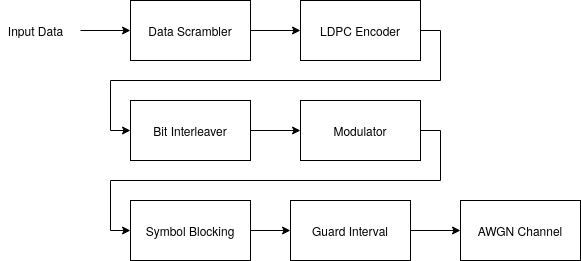
\includegraphics[scale=.4]{./media/phy.png}}
\caption{Transmitter block diagram for the DMG SC-PHY specification in IEEE 802.11ad}
\label{phy}
\end{figure}
\section{System Architecture}
A single frame consists of a short-training field (STF), a channel estimation field (CEF), a header and the data field. 
\subsection{Frame Structure}The STF consists of 16 repetitions of Golay sequences, $Ga_{128}(n)$ of length 128, followed by a single repetition of $-Ga_{128}(n)$. The CEF is used for channel estimation, as well as indication of which modulation is
going to be used for the packet. The CEF is composed of a concatenation of two
sequences Golay sequences, $Gu_{512}(n$) and $Gv_{512}(n)$, where the last 128 samples of $Gu_{512} (n)$ and $Gv_{512} (n)$ are equal to the last
128 samples used in the STF. They are followed by a 128 samples sequence $Gv_{128}(n)$ equal
to the first 128 samples of both $Gv_{512}(n)$ and $Gu_{512}(n)$. The CEF is pictured below in Fig. \ref{cef}
\begin{figure}[htbp]
\centerline{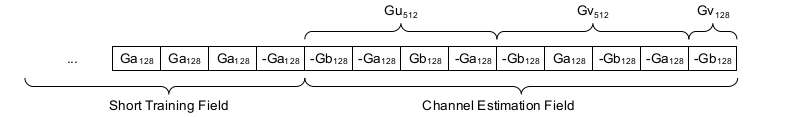
\includegraphics[scale=.35]{./media/cef.png}}
\caption{Channel estimation field for SC}
\label{cef}
\end{figure}


The header is fixed in length and comprised of twelve fields. The data field is is made up of the message bits, split up into blocks. 
\begin{figure}[htbp]
\centerline{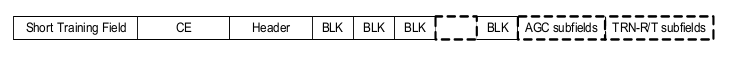
\includegraphics[scale=.35]{./media/frame.png}}
\caption{Frame structure for IEEE802.11ad}
\label{phy}
\end{figure}


The AGC and TRN-R/T subfields are used for power and synchronization. We don't implement these fields, as they are optional according to the specification.
\subsection{Data Scrambler} 
The header and data fields following the scrambler initialization field are scrambled by XORing each bit in turn with a length 127 periodic sequence generated by the polynomial
$S ( x ) = x^7 + x^4 + 1$. This is realized using a linear feedback shift register (LFSR) structure. The seed value is set randomly and added unscrambled as the seven bits of the header field for the receiver.
\begin{table*}[t]
\normalsize
\caption{802.11ad modulation and coding schemes}
\label{mcs}
\centering
\begin{tabular}{@{}cccccc@{}}
\toprule
MCS Indecx & Modulation & $N_{cbps}$ & Repetiton & Code Rate & Data Rate (Mbps) \\ \midrule
1 & $\pi/2$ BPSK & 1 & 2 & 1/2 & 385 \\
2 & $\pi/2$ BPSK & 1 & 1 & 1/2 & 770 \\
3 & $\pi/2$ BPSK & 1 & 1 & 5/8 & 962.5 \\
4 & $\pi/2$ BPSK & 1 & 1 & 3/4 & 1155 \\
5 & $\pi/2$ BPSK & 1 & 1 & 13/16 & 1251.25 \\
6 & $\pi/2$ QPSK & 4 & 1 & 1/2 & 1540 \\
7 & $\pi/2$ QPSK & 4 & 1 & 5/8 & 1925 \\
8 & $\pi/2$ QPSK & 4 & 1 & 3/4 & 2310 \\
9 & $\pi/2$ QPSK & 4 & 1 & 13/16 & 2502.5 \\ \bottomrule
\end{tabular}
\end{table*}
\subsection{Encoding}
The data are encoded by a systematic LDPC encoder. The LDPC is a block code. Each block of information
bits $(b_1 , b_2 ,...,b_k )$ is concatenated with a block of parity bits $(p_1 ,p_2 ,....,p_{n-k} )$ to create a codeword $c =( b_1 ,b_2 ,...,b_k ,p_1 ,p_2 ,....,p_{ n-k} )$ such that $Hc^T = 0$ , where $H$ is the (n-k)xn party check matrix. The block size n is $L_{CW}= 672$ bits. The code rate, $R$, is equal to $k/n$. 

Regarding the data, the LDPC encoding scheme depends on the repetition rate. If the repetition rate is $1$, the output stream of the scrambler is broken into blocks of $L_{CWD} = L_{CW} \times R$ bits. To each data word, $n-k=L_{CW} - R \times L_{CW}$ parity bits are added to create a codeword $c^{m}$ (the $m$th word), such that $Hc^{m^{T}} = 0$. If the repetition rate is $2$, then the data bits in each code word are concatenated with $L_{cw}/4$ zeros. The LDPC codeword $c$ is created by generating the parity bits  such that $Hc^T = 0$ , where $H$ is the parity matrix
for rate 1/2 LDPC code. Finally, we replace bits $L_{cw}/4 + 1$ through 336 of the codeword c with bits from the sequence XORed by a PN sequence that is generated from the LFSR used for data
scrambling as defined. The LFSR is initialized to the all ones vector and reinitialized to the same vector after every codeword. Regardless of repetition rate, the coded bits then are concatenated together and padded. 

The header is encoded separately from the data bits. The input header bits are scrambled, starting at the eighth bit. The LDPC codeword $c$ is generated by concatenating the header with the appropriate amount of zeros, such that $Hc^T = 0$, where $H$ is the parity check matrix for a rate $3/4$ code. The header is then split up into two sequences, one of which is XORed with a PN sequence from the LFSR, initialized to the all ones vector. The two sequences are then concatenated together to form the encoded header bits. For each of the different code rates, the standard specifies a different parity check matrix $H$.

\subsection{Modulation, Blocking and Guard Intervals} 
The STF and CEF are modulated as $\pi/2$ BPSK. The data field is modulated in ordinance with the specific modulation and coding scheme, either $\pi/2$ BPSK or $\pi/2$ QPSK. 
In $\pi/2$-BPSK modulation, modulation, the input bit stream is mapped according to the following equation: \begin{equation}
\tilde{s}_k = 2c_k - 1
\end{equation}where $c_k$ is the kth input coded (or scrambled pad) bit. Each output symbol is then rotated according to the following equation: 
\begin{equation}
s_k = \tilde{s_k}e^{ j \pi  k / 2 }
\end{equation}


In $\pi/2$-QPSK modulation, the input bit stream is grouped into sets of 2 bits and mapped according to the
1
following equation: 
\begin{equation}
\tilde{s_k} = \frac{1}{\sqrt{2}}((2c_{2k}-1)+j(2c_{2k+1}-1))exp(-j\frac{\pi}{4})
\end{equation}
where $k$ is the output symbol index, $k=0,1,\hdots$. Each output symbol is rotated according to the following equation
\begin{equation}
s_k = \tilde{s_k}e^{j\pi k/2}
\end{equation}
Depending on the symbol mapping, a guard interval made of a 64 bit Golay sequence is inserted into the data field. For example, for $\pi/2$ BPSK, the number of coded bits per block ($N_{cbpb}$) is 448. Fig. \ref{data} illustrates the insertion of the guard intervals for this case. 
\begin{figure}[htbp]
\centerline{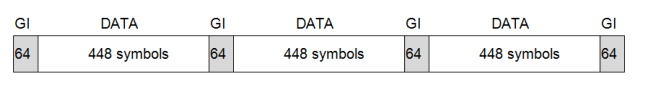
\includegraphics[scale=.4]{./media/data.png}}
\caption{Block transmission for $pi/2$ BPSK}
\label{data}
\end{figure} 

The two code words in the header field are blocked, an a 64 bit Golay sequence is placed between the two. The header is then modulated as $\pi/2$ BPSK. 

\section{Modulation and Coding Schemes}
We simulated the modulation and coding schemes, presented in Table \ref{mcs}. For a transmitter or receiver to comply to the standard, only MCSs 1-4 must be implemented, all others are beyond the scope of what is required in the specification.
% Please add the following required packages to your document preamble:
% \usepackage{booktabs}


MCS 1 is typically designated for a control channel, whereas all other MCSs are used for high bit-rate data transmission. 



\section{Simulations and Results} 
We simulated each of the specified MCSs over an AWGN channel to compute bit error rate curves. The standard was designed for high data rate communications, and uses extensive error correction, so simulating takes an extensive amount of computational time. 

In the simulation, we construct a frame consisting of modulated and coded CEF, STF, header and data fields. We then pass the frame through a wireless channel, and then recover the data field at the receiver. 

We simulated the transmission of ten frames, each consisting of 1000 data octets, corresponding to 8000 data bits per frame. For each frame, we computed the bit error rate over a range of signal-to-noise ratios for an AWGN channel. We scaled the channel noise accordingly to the modulation order and code rate. We then averaged the bit error rates over the ten packets to compute curves. 

In Fig. \ref{bpsk}, we show the BER curves for MCS1-5, which all use a $\pi/2$ BPSK modulation scheme. As expected, for higher MCS indices, corresponding to higher data-rates, there are more bit errors. Even at $-2$dB SNR, due to the repetition coding in MCS1, there were nearly no bit errors. This makes sense, since the control channel should be particularly robust. All in all, this implementation is rather performant, achieving very low bit error rates at low SNR values. 


\begin{figure}[htp]
\centerline{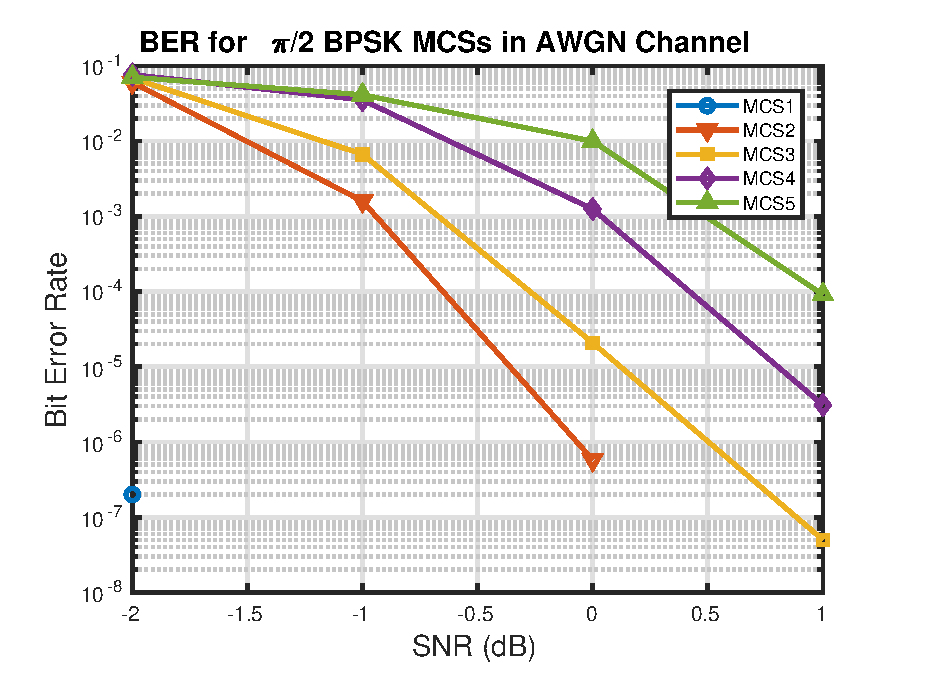
\includegraphics[scale=.6]{./media/bpsk.eps}}
\caption{BER curves for MCSs that use $\pi/2$ - BPSK modulation}
\label{bpsk}
\end{figure} 

In Fig. \ref{qpsk}, we illustrate the performance of MCS6-9 via BER curves. Again, these curves highlight the robustness of the specification to AWGN channels. This makes sense, given that the standard is designed for short-range, high throughput communications. Over such short ranges, fading and multi-path channels can provide severe attenuation, necessitating the use of LDPC codes to ensure that a high level of QoS is maintained.  

\begin{figure}[htp]
\centerline{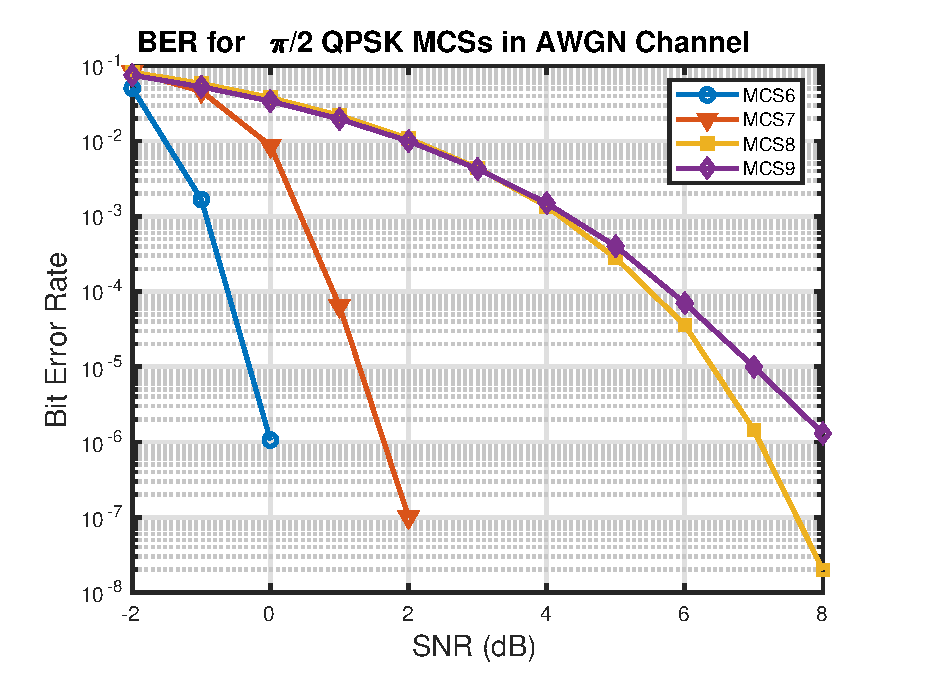
\includegraphics[scale=.6]{./media/qpsk.eps}}
\caption{BER curves for MCSs that use $\pi/2$ - QPSK modulation}
\label{qpsk}
\end{figure} 



\section{Conclusion} 
We successfully studied, implemented and simulated a portion of the DMG SC-PHY layer of the IEEE802.11ad standard. We sucessfully transmitted a frame in ordinance with the specifcation, and appropritely decoded the data bits to compute BER curves. We were able to see how the combination of LDPC codes, gaurd intervals, golay and PN sequences and various modulation schemes worked in tandem allow for high, multi-gigabit data rates in a wireless system. We demonstrate that the standard achieves very low bit error rates at low SNR values, making the standard appropriate for in-house wireless virtual reality, video gaming, movie and music streaming. 

\bibliographystyle{unsrt}
\bibliography{bibli}
\end{document}